\documentclass[journal]{IEEEtran}
\usepackage{blindtext}
\usepackage{graphicx}
\usepackage{hyperref}
\usepackage{dcolumn}% Align table columns on decimal point
\usepackage{bm}% bold math
\usepackage{amsmath}
\usepackage{mathtools}
%\usepackage{todonotes}
%\usepackage{booktabs}
\usepackage{colonequals}
\usepackage{ulem}
\usepackage{amssymb}
\usepackage{color}
\usepackage{algorithm}
\usepackage[noend]{algpseudocode}
% steve's notes
\newcommand{\srN}[1]{\todo[inline, size=\small, color=cyan!30]{[sr] #1}}
\newcommand{\srn}[1]{\todo[color=cyan!30]{[sr] #1}}

\hyphenation{op-tical net-works semi-conduc-tor}


\begin{document}

	\title{On the Entropy and Divergence of Gaussian Mixture Models}

	
	\author{Diego~Granziol and~Stephen~Roberts% <-this % stops a space
		\thanks{Machine Learning Research Group, University of Oxford}% 
	}
	


	\maketitle
	
	
	\begin{abstract}
		%\boldmath
		
For the widely applied and practical Gaussian mixture model (GMM), there exists no closed form expression for the differential entropy. We derive a novel upper bound for the differential entropy of a GMM using the method of maximum entropy and propose an algorithm for its calculation. We further show that the Kullback Leibler (KL) divergence between two GMM's can be trivially estimated using the parameters of its .
		
	\end{abstract}

	\begin{IEEEkeywords}
		Gaussian mixtire models, differential entropy, KL divergence, Maximum entropy methods.
	\end{IEEEkeywords}
	

	\IEEEpeerreviewmaketitle
	\section{Introduction}
Differential entropy, defined as $\int p(x)\log p(x)dx$ \cite{cover2012elements} extends the notion of classical entropy \cite{shannon2001mathematical} to continuous measures. In the case of bounded measures, or for those for which it makes sense to propose a uniform prior \cite{caticha2012entropic}, it has a natural interpretation as uncertainty over the density $p(x)$, reaching a maximum for the uniform and a minimum for the Dirac delta distribution. It is used for parameter estimation \cite{cheng1983estimating}	and for the computation of mutual information (MI). \begin{equation}
\text{MI} = \int p(x,y)\log \frac{p(x,y)}{p(x)p(y)}dxdy
\end{equation} This is an ubiquitous term, meausing the Kullback-Leiber divergence between a joint density and its marginals. It is used in in a variety of applications, such as communication channel capacity \cite{cover2012elements}, sensor management \cite{manyika1992information} and image restoration \cite{viola1997alignment}. \newline The Kullback-Leiber divergence \cite{cover2012elements}, also known as the relative entropy, or minimum discrimination information, between two densities $f(x)$ and $g(x)$ is defined as \begin{equation}
\mathcal{D}_{kl}(f||g) = \int f(x)\log \frac{f(x)}{g(x)}dx
\end{equation}
and satisfies the properties of

\begin{enumerate}
	\item Self Similarity: $\mathcal{D}_{kl}(f||f) = 0$
	\item Self Identification: $\mathcal{D}_{kl}(f||g) = 0\thinspace  \text{iff} \thinspace f=g$
	\item Positivity: $\mathcal{D}_{kl}(f||g) \geq 0 \thinspace \forall f,g$
\end{enumerate}
It is widely applied as a similarity measure for speech \cite{olsen2003efficient}, image, text \cite{huo2006dtw} and HMMs \cite{silva2006average}. Futhermore, its Hessian defines the Fisher-Rao metric, which allows us to define a unique Riemmanian manifold, on which the points corresponds to probability measures and from which we can calculate informational difference between measurements \cite{amari2007methods}.
\section{Entropy, KL and Gaussian Mixture Models}
For Gaussian distributions both the differential entropy and KL divergence have closed form solutions. However for highly skewed or multimodal distributions which describe real world data, the Gaussian approximation may be in-appropriate. The Gaussian mixture (where $\sum w_{i}=1$)
\begin{equation}
\text{GMM} = \sum_{i}^{N}w_{i}\mathcal{N}(\vec{x};\vec{\mu_{i}},\vec{\Sigma_{i}})
\end{equation}  is a widely adopted and practical universal function approximator \cite{maz1996approximate}, used to deal with the short comings of the single Gaussian. Unfortunately for the GMM, due to the summation term in the logarithm, no analytic expression of the differential entropy or the KL divergence between two GMM's exists. 
\section{related work}
In \cite{huber2008entropy} the authors propose an analytical approximation to the differential entropy, by using the GMM moments and truncating the logarithm expansion after $R$ terms
\begin{equation}
\begin{aligned}
& H(\vec{x}) \approx  -\sum_{i}^{N}\int_{\mathbb{R}^{n}}w_{i}\mathcal{N}(\vec{x};\vec{\mu_{i}},\vec{\Sigma_{i}})\\
& \times \biggr(\sum_{k=0}^{R}\frac{1}{k!}\bigg((x-\mu_{k})\odot\nabla\bigg)^{k}\log g(x)\bigg\rvert_{x=\mu_{i}}\biggr)\\
\end{aligned}
\end{equation}
Where $\odot$ stands for the matrix contraction operator. They further derive an upper bound to the GMM differential entropy
\begin{equation}
H_{u1} = \sum_{i}^{N}-w_{i}\log w_{i} + \frac{1}{2}\log((2\pi e)^{N}|\Sigma_{i}|)
\end{equation}
In \cite{hershey2007approximating} they propose and compare a variety of approximations to the computationally demanding gold standard of Monte Carlo simulation. They propose to replace the full GMM density $p(x)$ with either a single or product of Gaussian(s) in order to calculate the KL divergence. They further propose and finally conclude in favour of their analytical variational approximation
\begin{equation}
\mathcal{D}_{var}(f||g) = \sum_{a}\pi_{a}\log \frac{\sum_{a'}\pi_{a'}e^{-\mathcal{D}(f_{a}||f_{a'})}}{\sum_{b}w_{b}e^{-\mathcal{D}(f_{a}||g_{b})}} 
\end{equation}
where $\pi_{a}$ represents the weight of the $a$'th Gaussian component in mixture $f$ and $f_{a}$ corresponds to that density. {\color{red}{check this}}
	\section{Contributions of this Paper}
In this paper, we use the method of maximum entropy and the moments of the GMM to derive a novel upper bound on the GMMs differential entropy and a novel approximation to the KL divergence between two GMMs. The structure of the paper is as follows
\begin{itemize}
\item We prove that the power moments of a GMM completely define its characteristic function and hence its density. This establishes the validity of using the GMMs power moments to estimate a more tractable surrogate density. 
\item We use the distribution of maximum entropy given the GMM's moments as constraints to upper bound the differential entropy of the GMM
\item We prove, using the non-negativity of the multivariate mutual information \footnote{There are many variants of the multivariate mutual information, some of which can be negative, we propose a natural definition of what we call the dependence information, which is non-negative} that the entropy of the multivariate distribution of maximum entropy is a lower bound to the sum of entropies of the univariate (marginal) distributions of maximum entropy
\item This allows us to avoid computing computationally costly multi-dimensional numerical integrations, reducing an $n^{d}$ numerical integration to $n\times 1^{d}$ numerical integrations.
\item We propose an algorithm written in Python for the computation of an upper bound of the differential entropy of a GMM, make the code available and compare it to various other approximations in the literature
\item We further show how the parameters of the distribution of maximum entropy allow for an approximate calculation of the KL divergence between two GMMs and compare it to other approximations in the literature
\end{itemize}



	\section{Maximum Entropy}
The method of maximum entropy (MaxEnt) \cite{maxentreview} is a method which generates the least biased estimate of a proposal probability distribution, $q(x)$, given information in the form of functional expectations (also known as constraints). It is maximally non-committal in regards to missing information \cite{inftheoryjaynes}. Mathematically we maximize the functional,
\begin{equation}
\label{BSG}
S = \int q(\vec{x})\log q(\vec{x})d\vec{x}- \sum_{i}\lambda_{i}\bigg[\int p(\vec{x})f_{i}(\vec{x})d\vec{x} - \mu_{i}\bigg],
\end{equation}
with respect to $q(\vec{x})$, where $\langle f_{i}(\vec{x})\rangle = \mu_{i}$ are the values of the imposed mean value constraints. For stochastic trace estimation, the functions are the power moments, $f_{i} = x^{i}$. The first term in Equation \eqref{BSG} is the Boltzmann-Shannon-Gibbs (BSG) entropy. This has been applied in a variety of disparate fields, from modelling crystal defects in lattice models in condensed matter physics \cite{giffin} to inferring asset price movement distributions from option prices in finance \cite{nerioptions,entropybuchen}. It can be used to derive statistical mechanics (without the a priori assumptions of ergodicity and metric transitivity \cite{diego}), non-relativistic quantum mechanics, Newton's laws and Bayes' rule \cite{Gonzalez2014,caticha2012entropic}. It can be proved under the axioms of consistency, uniqueness, coordinate invariance, subset and system independence, that for mean value constraints any self consistent inference scheme must either maximize the entropic functional \eqref{BSG}, or any functional sharing its maximum \cite{shore1980axiomatic,maxentreview}. The Johnson and Shore axioms state that the entropy must have a unique maximum \cite{shore1980axiomatic} and, given the convexity of the BSG entropy, it contains a unique maximum provided that the constraints are convex. This is satisfied for any polynomial in $x$ and hence entropy maximization, given moment information, constitutes a self consistent inference scheme \cite{maxentreview}.
	
	\section{Are moments sufficient to fully describe the problem?}
	\label{momentsanddistributions}
	For a probability measure $\mu$ having finite moments of all orders $\alpha_{k} = \int_{-\infty}^{\infty} x^{k}\mu(dx)$, if the power series $\sum_{k}\alpha_{k}/k!$ has a positive radius of convergence, that $\mu$ is the only probability measure with the moments $\alpha_{1},\alpha_{2},...$ \cite{billingsley_2012}. \newline Informally, a Gaussian has finite orders of all moments, hence any finite combination of Gaussians must necessarily possess finite moments of all orders and the above condition is satisfied.
	\newline For the case of a one dimensional Gaussian with a location parameter $\mu_{i}$ and standard deviation $\sigma_{i}$ it can be seen that the $2k$'th moment
	\begin{equation}
	G_{2k} = \sum_{2p=0}^{2k} {2k\choose 2p} \mu_{i}^{2(k-p)}\beta_{i}^{-p}
	\end{equation}
	As all odd power moments of the Gaussian are 0. Hence for the Gaussian mixture model we have
	\begin{equation}
	GMM_{2k} = \sum_{i=1}^{N}w_{i}\sum_{2p=0}^{2k} {2k\choose 2p} \mu_{i}^{2(k-p)}\beta_{i}^{-p}
	\end{equation}
	We note that since $\sum_{i} w_{i} = 1$ and $w_{i}\geq 0$ that $w_{i}\leq 1$. Furthermore $\mu_{i} \leq \mu_{upper} > 1 \thinspace $ and $\beta_{i} \geq \beta_{lower} < 1$ $\forall i$. We can bound the above expression by further seeing that $\sum_{2p=0}^{2k} {2k\choose 2p} < (k+1)\frac{(2k)!}{(k!)^{2}}$. Hence
	\begin{equation}
	GMM_{2k} < N(k+1)\frac{(2k)!}{(k!)^{2}(\mu_{max}^{2k}\beta_{i}^{-k})}
	\end{equation}
	Which we can see is smaller than $(2k)!$ in the $k\rightarrow \infty$ limit by taking logarithms
	\begin{equation}
	\frac{\log N}{2k} + \frac{\log(k+1)}{2k} + \log mu_{max} + \frac{|\log \beta_{i}|}{2} \leq \log k 
	\end{equation} 
 

	\section{Proof of MaxEnt proposal as an upper bound}
	\label{mainresults}
	Consider the KL divergence $\mathcal{D}_{kl}$, \cite{cover2012elements} between the true Gaussian mixture density $p(x)$ and a proposal MaxEnt solution $q(x) = \exp(\sum_{j}\alpha_{j}x^{i})$:
	\begin{equation}
	\label{kldiv}
	\mathcal{D}(P||Q) = \int p(x)\log p(x)dx - \int p(x)\log q(x) 
	\end{equation} note that the (self) entropy of the MaxEnt solution is given by
	\begin{equation}
	\begin{aligned}
	\label{ent1}
	& H(Q) = -\int q(x)\log q(x) dx \\
	&= \sum_{i}\alpha_{i}\int x^{i}\exp\bigg(-\sum_{j}\alpha_{j}x^{j}\bigg)dx = \sum_{i}\alpha_{i}\langle x^{i} \rangle,
	\end{aligned}
	\end{equation}
	where $\alpha$ denotes the Lagrange multipliers pertaining to the MaxEnt solution and $\langle x^{j} \rangle$ refers to the expectation of the $j^{\text{th}}$ moment. 
	
	The first term in equation \eqref{kldiv} is the (unknown) negative entropy of the GMM $\mathcal{S}(p)$. We can thus rewrite equation \eqref{kldiv} as:
	\begin{equation}
	\label{sumentropies}
	\begin{aligned}
	&-H(P) + \int p(x)\sum_{i}\alpha_{i}x^{i} = -H(P) + \sum_{i}\alpha_{i}\langle x^{i} \rangle \\
	& = -H(P) + H(Q).
	\end{aligned}
	\end{equation} 
	Where we have used the fact that the functional expectations of our MaxEnt distribution by construction (Equation \eqref{BSG}) match that of the underlying distribution.  Using the information inequality \cite{cover2012elements} it is clear, that the entropy of our proxy MaxEnt solution serves as an upper bound to that of the true solution, i.e.
	\begin{equation}
	\label{dataprocessesing}
	\mathcal{D}_{kl}(P||Q) = H(Q) -H(P) \geq 0 \rightarrow H(Q) \geq H(P).
	\end{equation}
	
\section{Multidimensional Entropy}
For an $n$ dimensional variable, we can define a variant of the mutual information as
\begin{equation}
I_{d}(x_{1}.....x_{n}) \equiv \int p(x_{1}.....x_{n})\log \frac{p(x_{1}.....x_{n})}{\prod_{i}^{n}p(x_{i})}\prod_{i}^{n}dx_{i}
\end{equation}
Which we denote as the dependence information. This can be split into a sum of entropic terms 
\begin{equation}
I_{d}(x_{1}.....x_{n}) = -H(x_{1}...x_{n}) + \sum_{i}^{N}H(x_{i})
\end{equation}
and is thus seen to measure the difference in entropy between the joint and the sum of the entropies of the marginals, justifying its name.
\newline It can be easily shown using the convexity of the negative log function and Jensens inequality ($\mathbb{E}[f(x)]\geq f[\mathbb{E}(x)]$) that
\begin{equation}
\begin{aligned}
& -\int p(x_{1}..x_{n})\log \frac{\prod_{i}^{n}p(x_{i})}{p(x_{1}...x_{n})}\prod_{i}^{n}dx_{i} \geq -\log\int \prod_{i}^{n}p(x_{i})dx_{i}\\
& \therefore I_{d}(x_{1}.....x_{n}) \geq 0 \\
& \therefore \sum_{i}^{N}H(x_{i}) \geq H(x_{1}...x_{n}) \\
\end{aligned}
\end{equation} 
Note that this is different to the interaction information \cite{mcgill1954multivariate} or conditional mutual information, which are defined (for the case of $3$ variables) as
\begin{equation}
I(x_{1},x_{2},x_{3}) = -\sum_{i}H(x_{i})+\sum_{i\neq j}H(x_{i},x_{j})-H(x_{1},x_{2},x_{3}))
\end{equation}
With a differing sign convention for odd variables. This type of multivariate mutual information can be negative. \newline It is thus clear that we can reduce the problem of multi-variate GMM differential entropy estimation, to that of a sum of uni-variate GMM differential entropy estimation, for which we can apply numerical techniques such as quaderature and sampling in a computational efficient manner to solve the problem of Maximum entropy. Formally for an $n$ dimensional GMM
\begin{equation}
H(x_{1}...x_{n}) \leq \sum_{i}^{n}H(x_{i}) \leq \sum_{i}^{n}\mathcal{S}(x_{i})
\end{equation}
Where $H(x)$ denotes the entropy,of the joint and the marginals respectively and $\mathcal{S}$ denotes the surrogate density of maximum entropy. In the case of the GMM
\begin{equation}
GMM(\vec{x}) = \sum_{i}\frac{w_{i}}{\sqrt{(2\pi)^{k}\Sigma_{i}}}\exp\bigg((\vec{x}-\vec{\mu_{i}})^{t}\Sigma^{-1}_{i}(\vec{x}-\vec{\mu_{i}})\bigg)
\end{equation}

we have an analytic expression for the marginal densities $p(x_{i})$, where we simply drop the terms from the mean vector and covariance matrix, as can be shown by the definition of the multivariate normal and linear algebra and hence
\begin{equation}
GMM(x) = \sum_{i}\frac{w_{i}}{\sqrt{(2\pi)\sigma_{i}}}\exp\bigg(\frac{(x-\mu_{i})^{2}}{2\sigma_{i}^{2}}\bigg)
\end{equation}

\section{KL divergence between two GMMs}
Consider two GMMs with true underlying density $p_{1}(x)$ and $p_{2}(x)$ and their Maximum Entropy surrogates $q_{1}(x)$ and $q_{2}(x)$, Then it is easy to see that
\begin{equation}
\mathcal{D}_{kl}(p_{1}||p_{2}) \approx \int q_{1}(x) \log \frac{q_{1}(x)}{q_{2}(x)}dx
\end{equation}
Writing $q_{1}(x) = \exp(\sum_{i}\alpha_{i}x^{i})$ and $q_{2}(x) = \exp(\sum_{j}\lambda_{j}x^{j})$
\begin{equation}
\mathcal{D}_{kl}(p_{1}||p_{2}) \approx \mathcal{S}(p_{1}) - \sum_{j}\lambda_{j}\mathbb{E}_{p_{2}}(x^{j})
\end{equation}
Extending this notion to higher dimensions, we consider the surrogate to be the product of its maximally entropic marginals and hence we arrive at for an $n^{d}$ GMM where we take 40 moments of its marginals
\begin{equation}
\mathcal{D}_{kl}(p_{1}(\vec{x})||p_{2}(\vec{x})) = -\sum_{i}^{n}\mathcal{S}(x_{i})+\sum_{i}^{n}\sum_{j}^{m}\lambda_{i,j}\mathbb{E}_{p_{2}}(x^{j}_{i})
\end{equation}
	\section{Lagrangian Duality}
	Consider a generic optimization problem of the form,
	\begin{equation}
	\begin{aligned}
	&\text{minimize } \thinspace f_{0}(x)\\
	&\text{subject to } \thinspace f_{i}(x) \leq 0, \thinspace i=1...m\\
	&\text{subject to } \thinspace h_{i}(x) = 0, \thinspace i=1...p
	\end{aligned}
	\end{equation}
	where $x \in \mathbb{R}^{n}$ and the domain $\mathcal{D} = \bigcap\limits_{i=0}^{m} f_{i}\cap\bigcap\limits_{i=1}^{p}h_{i}$. We define the Lagrangian dual function as the infimum of the Lagrangian over the domain of $x$,
	\begin{equation}
	\begin{aligned}
	& g(\lambda,\nu) = \underset{x \in \mathcal{D}}{\mbox{inf}}L(x,\lambda, \nu)\\
	& = \underset{x \in \mathcal{D}}{\mbox{inf}}\bigg( f_{0}(x) + \sum_{i=1}^{m}\lambda_{i}f_{i}(x) + \sum_{i=1}^{p}\nu_{i}h_{i}(x)\bigg).
	\end{aligned}
	\end{equation}
	As the dual is the pointwise infimum of a family of affine functions of $(\lambda, \nu)$, it is concave, irrespective of the convexity of $f_{0},f_{i},h_{i}$. \cite{boyd_vandenberghe_2009}. It is easily verifiable due to the net negativity of the two summation terms in $g(\lambda, \nu)$ that the dual provides a lower bound on the optimal value $p^{*}$ of the primal problem. This is known as weak duality. In the case of equality constraints this bound is tight. 
	
	For general inequality constraints the difference between the primal and dual optimal solution (duality gap) is not 0. However, for $f_{0}...f_{m}$ convex, Affine equality constraints and certain regularity conditions, we have a duality gap of $0$, this is known as strong duality. An example of such a constraint qualification is Slater's condition, which states that there is an $x \in \mbox{rel. int. } (\mathcal{D})$ which satisfies the constraints (where rel. int. refers to the relative interior).

	\subsection{Application to Maximum Entropy}
	\label{entropydecreaseproof}
	We wish to maximise the entropic functional $\mathcal{S}(p) = -\int p(x)\log p(x)dx$ under certain moment constraints $\int p(x)x^{m}dx = \mu_{m}$. This can be written as,
	\begin{equation}
	\begin{aligned}
	&\text{minimize } \thinspace f_{0}[p(x)] = \int p(x)\log p(x)dx\\
	&\text{subject to } \thinspace h_{i}[p(x)] = \int p(x)x^{i}dx - \mu_{i} = 0, \thinspace i=1...p.
	\end{aligned}
	\end{equation}
	Given that the negative entropy is a convex objective and that the moment equality constraints are affine in the variable being optimised over $p(x)$ by strong duality we have an equivalence between the solution of the dual and that of the primal.
	
	It is also clear that the domain defined as the intersection of the constraint sets can never increase upon the addition of an extra constraint. Hence,
	\begin{equation}
	\underset{x \in \mathcal{D}=\bigcap\limits_{i=0}^{m}f_{i}}{\mbox{inf}}L(x,\lambda, \nu) \leq \underset{x \in \mathcal{D}=\bigcap\limits_{i=0}^{m+1}f_{i}}{\mbox{inf}}L(x,\lambda, \nu)
	\end{equation}
	and thus the entropy can only decrease when adding an extra constraint. Hence by adding more moment constraints, we always reduce the entropy and given equations \eqref{dataprocessesing} and \eqref{sumentropies} we necessarily reduce $\mathcal{D}_{kl}(p[x]||q[x])$, where $p[x], q[x]$ define the true eigenvalue and MaxEnt proposal distributions respectively.
	
	\section{Algorithm}
	We apply a numerically stable MaxEnt Algorithm (algorithm \ref{alg:coefopt}) \cite{bandyopadhyay2005maximum}, under the conditions that $\lambda_i$ is strictly positive and the all power moments $0 \leq \lambda^{k}\leq 1$. 
	We can satisfy these conditions by normalizing our positive definite matrix by the maximum of the Gershgorin intervals~\cite{Gershgorin1931}.
	
	\algrenewcommand\algorithmicindent{1.3em}
	\renewcommand{\algorithmicrequire}{\textbf{Input:}}
	\renewcommand{\algorithmicensure}{\textbf{Output:}}
	
	\begin{algorithm}
		\caption{Optimising the Coefficients of the MaxEnt Distribution}\label{alg:coefopt}
		\begin{algorithmic}[1]
			\vspace{0.5em}
			\Require Moments $\{\mu_i\}$, Tolerance $\epsilon$ 
			\Ensure Coefficients $\{\alpha_i\}$
			\State $\alpha_i \sim \mathcal{N}(0,1)$
			\State $i \gets 0$
			\State $p(\lambda) \gets \exp(-1 - \sum_k \alpha_k \lambda^k)$
			\While{error $< \epsilon$}
			\State $\delta \gets \log \left(\frac{\mu_i}{\int \lambda^i p(\lambda) d\lambda} \right)$
			\State $\alpha_i \gets \alpha_i + \delta$
			\State $p(\lambda) \gets p(\lambda | \alpha)$
			\State error $\gets \max |\int \lambda^i p(\lambda) d\lambda - \mu_i|$
			\State $i \gets \text{mod}(i+1, \text{length}(\mu))$
			\EndWhile 
		\end{algorithmic}
	\end{algorithm}
	
	We follow the procedure from entropic trace estimation \cite{ete}. Firstly, the raw moments of the eigenvalues are estimated using stochastic trace estimation. These moments are then passed to the maximum entropy optimization of Algorithm \ref{alg:coefopt} to produce an estimate of the distribution of eigenvalues, $p(\lambda)$.
	Consequently, $p(\lambda)$ is used to estimate the distribution's log geometric mean, $\int \log(\lambda) p(\lambda) d\lambda$.
	This term is multiplied by the matrix's dimensionality and if the matrix was normalized, the log of this normalization term is added. We lay out these steps more concisely in Algorithm \ref{alg:logdet}.  
	
	\algrenewcommand\algorithmicindent{1.3em}
	\renewcommand{\algorithmicrequire}{\textbf{Input:}}
	\renewcommand{\algorithmicensure}{\textbf{Output:}}
	
	\begin{algorithm}
		\caption{Entropic Trace Estimation for Log Determinants}\label{alg:logdet}
		\begin{algorithmic}[1]
			\vspace{0.5em}
			\Require PD Symmetric Matrix $A$, Order of stochastic trace estimation $k$, Tolerance $\epsilon$
			\Ensure Log Determinant Approximation $\log|A|$
			\State $B = A/\|A\|_2$
			\State $\mu$ (moments)$ \gets$ StochasticTraceEstimation$(B, k)$ 
			\State $\alpha$ (coefficients) $\gets \text{MaxEntOpt(}\mu, \epsilon)$
			\State $p(\lambda) \gets p(\lambda | \alpha)$
			\State $\log|A| \gets n\int \log(\lambda) p(\lambda) d\lambda + n\log(\|A\|_2)$
		\end{algorithmic}
	\end{algorithm}
	
	\subsection{Algorithmic details for Practitioners}
	Given that the MaxEnt approach of Algorithm \ref{alg:coefopt} is numerical, we need to specify a gridding of the input space or choice of nodes. We find that a gridding between $0\leq x \leq 1$ of $\Delta x = 0.001$ provides a good trade-off between speed and accuracy, with essentially the same results (measured by absolute error) as $\Delta x = 0.0001$. We find that even when we set the tolerance $\epsilon$ in algorithm \ref{alg:coefopt} to $10^{-4}$ (smaller values than this significantly increase run time) the entropy, shown in Figure \ref{fig:thermoentropyvsmoments} and by the results of section \ref{mainresults}  the absolute error shown in Figure \ref{fig:thermomech1sampleerrorvsmoments} does not seem to decrease beyond $m \approx 10$ moments. We note that $\epsilon$ represents a maximum error to which extent each moment constraint can be violated. Given that the eigenvalue power moments are strictly decreasing, this means the higher order moment constraints can be violated by a greater relative fraction, which when combined with the fact that the constraints are noisy and that the computational complexity of cycling through all the constraints with an approximate correction term (the basis for algorithm \ref{alg:coefopt}) increases with more moments (as does the error per constraint) the usefulness of using more moment information is limited. We hence don't recommend using more than $10$ moments. It is also ill advised to use moment information which is smaller than your error tolerance.
	\begin{figure}[t]
		\centering 
		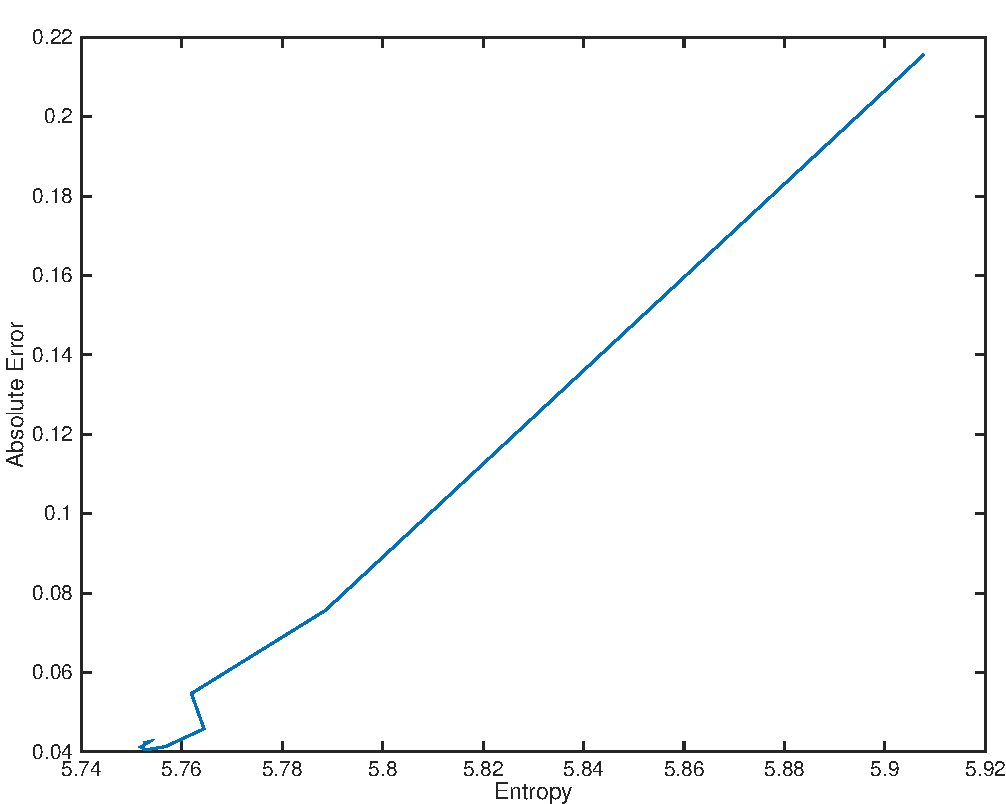
\includegraphics[width=0.5\textwidth]{thermoentr1smp-cropped}
		\caption{Relative error against entropy for a single sample stochastic trace estimate from 2 to 10 moments for the Thermomech dataset.}
		\label{fig:thermomech1sampleerrorvsentropy}
	\end{figure}
	\begin{figure}[t]
		\centering 
		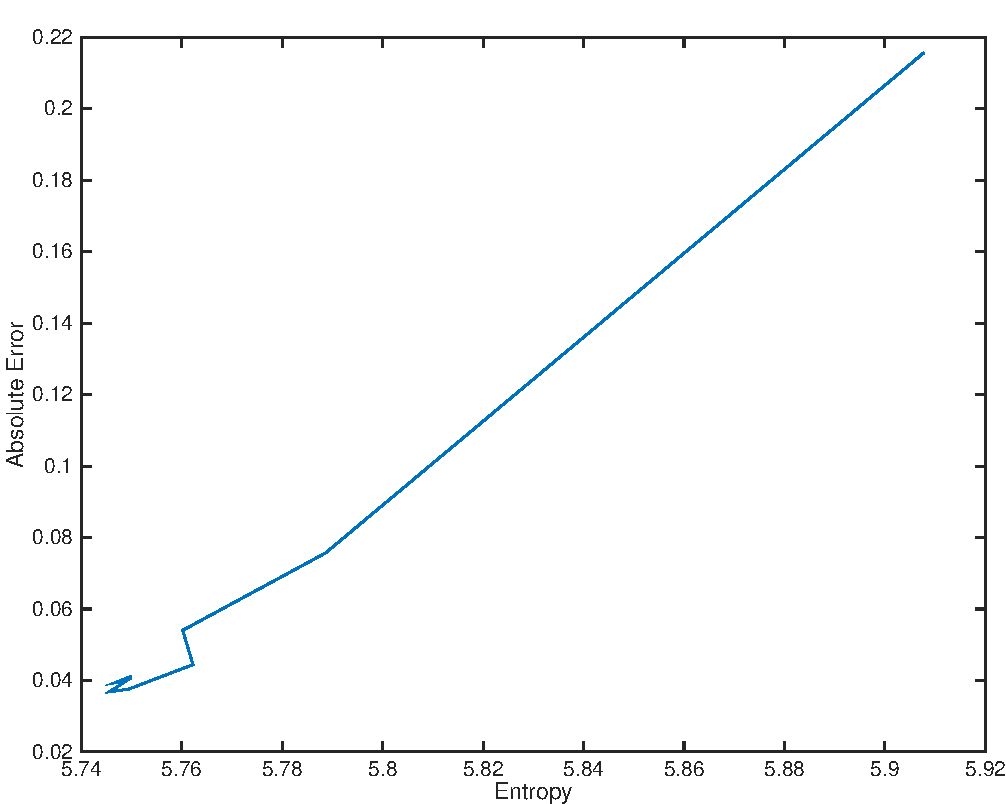
\includegraphics[width=0.5\textwidth]{thermo50smp-cropped}
		\caption{Relative error against entropy for a 50 sample stochastic trace estimate from 2 to 10 moments for the Thermomech dataset.}
		\label{fig:thermomech30sampleerrorvsentropy}
	\end{figure}
	
	\section{Stochastic trace estimates}
	A key component of the computational complexity of Entropic trace estimation \cite{ete}, is the number of stochastic samples taken. Hence we ask the question, how does the quality of our inference, i.e the approximation to the log determinant depend on the number of samples taken?
	
	To keep our results comparable and consistent, we keep with \cite{ete,bild} and consider Gaussian random unit vectors. We note that across a variety of sparse datasets, the number of samples taken neither largely effects the entropy of the proposal distribution (used to determine the number of moments required before attaining an optimal result) as is demonstrated by the indiscernability of Figures \ref{fig:thermomech1sampleerrorvsentropy} and \ref{fig:thermomech30sampleerrorvsentropy}, where we compare the Entropy of the corresponding MaxEnt distribution for $1$ of $50$ stochastic trace samples. For Figure \ref{fig:thermomech1sampleerrorvsmoments} the corresponding graph for $50$ stochastic samples is also virtually identical. Given this behaviour we empirically investigate the extent to which reducing the number of stochastic samples affects the estimation of the log determinant.
	
	
	\subsection{Single sample result comparisons}
	We load five sparse (SuiteSparse) square PSD matrices, ranging from a maximum dimension of $999,999$ to a minimum of $81,200$ and run Cholesky using the Matlab 2014b `Chol' function to calculate the log determinants on a 2.6 GHz Intel Core i7 16 GB 1600 MHz DDR3 notebook. This takes 4847 seconds. Using our MaxEnt Algorithm \ref{alg:coefopt}, with a gridding of $0.001$ and 30 stochastic samples of 8 moments, we calculate the log determinants in 20 seconds. For a single sample, we calculate the log determinants in 16 seconds.  The respective errors are shown in Table \ref{table:experiment 1}.
	\begin{table}[h!]
		\centering
		\begin{tabular}{||c c c c||} 
			\hline
			Dataset & Dimension & Samples & Error\\ [0.5ex] 
			\hline\hline
			ecology2 & 999,999 & 30 & 0.0102 \\
			&  & 1 & 0.0105\\
			\hline
			thermomech TC & 102,158 & 30 & 0.0398\\
			& 102,158 & 1 & 0.0402\\
			\hline
			shallow water 1 & 81,920 & 30 & 0.0043\\
			&  & 1 & 0.0035\\
			\hline
			shallow water 2 & 81,920 & 30 & 0.0039\\
			&  & 1 & 0.0040\\
			\hline
			apache1 & 80,800 & 30 & 0.006571\\
			&  & 1 & 0.0101\\ [0.5ex] 
			\hline
		\end{tabular}
		\newline
		\caption{Relative absolute error on SuiteSparse datasets, for 8 moments and 30/1 samples per moment}
		\label{table:experiment 1}
	\end{table}
	We note that even for relatively small matrices, $n \approx 80,000$, that the performance from reducing the number of samples is relatively unaffected. However, given that there is a slight decrease in performance and that 15 of the 20 and 16 seconds of compute time were spent on Alogorithm \ref{alg:coefopt}, determining the Maximum Entropy coefficients, we recommend reducing the number of samples only when it becomes a larger proportion of the overall cost. 
	
	We further test the performance impact, by evaluating the difference in MaxEnt estimate for the largest PSD matrices in the SuiteSparse data set, comparing a single sample to $30$ samples. For $\text{Queen}$ $ 4147$ with a dimension of $4,147,110$ and $316,548,962$ non zero values, the difference in prediction from taking $1$ sample instead of $30$ is $0.0028\%$ and the run-time is reduced from $173$ to $60$ seconds. We note that the standard Cholesky and LU functions in (e.g.) MATLAB are unable to handle matrices of that size, due to contiguous memory constraints, even on significantly more powerful machines than the one above. Table \ref{table:experiment 2} shows results for a variety of large datasets.
	\begin{table}[h!]
		\centering
		\begin{center}
			\begin{tabular}{||c c c c c c||} 
				\hline
				Dataset & Dimension & Samples & Estimate & Time(s)  & \textbf{$\Delta \%$} \\ [0.5ex] 
				\hline\hline
				Queen & 4,147,110 & 30 & -7.3951e+07 & 172.4 & \\
				Non 0's & 316,548,962 & 1 & -7.3953e+07 & 60.3 & 0.0028 \\ 
				\hline
				Bump & 2,911,419 & 30 & -5.2282e+07 & 64.3 &\\ 
				Non 0's & 127,729,899 & 1 & -5.2297e+07 & 15.9 & 0.029\\ 
				\hline
				Serena & 1,391,349 & 30 & -1.5831e+07 & 34.4 & \\ 
				Non 0's & 64,131,971 & 1 & -1.5771e+07 & 8.867 & 0.38\\ 
				\hline
				Geo & 1,437,960 & 30 & -1.0186e+07 & 33.2 &\\ 
				Non 0's & 60,236,322 & 1 & -1.0203e+07 & 12.5 & 0.17\\
				\hline
				Hook & 1,498,023 & 30 & -4.6026e+06 & 32.3 & \\  
				Non 0's & 59,374,451 & 1 & -4.6033e+06 & 11.8 & 0.015\\
				\hline
				StochF & 1,465,137 & 30 & -2.6807e+07 & 15.4 & \\ 
				Non 0's & 21,005,389 & 1 & -2.6812e+07 & 7.1 & 0.019\\
				\hline
				G3 & 1,585,478 & 30 & -1.0263e+07 & 9.875 & \\  
				Non 0's & 7,660,826 & 1 & -1.0262e+07 & 4.618 & 0.097 \\ [0.5ex] 
				\hline
			\end{tabular}
		\end{center}
		\caption{results for the largest psd suitesparse matrices, using 8 moments, with sample number either 30 or 1. Final column denotes percentage difference in estimate between using 30/1 sample(s).}
		\label{table:experiment 2}
	\end{table}
	The reduction in samples from $30$ to $1$ reduces the computational run-time by a factor of $3$ and the difference in estimates, which is always less than $0.4\%$ tends to increase in as the matrix dimension decreases. The exceptions, \textit{StochF} and \textit{G3}, are both significantly sparser than the others, which is why they run significantly faster and the MaxEnt calculation algorithm (which is independent of the number of samples taken) takes up a greater proportion of the total run-time and hence the reduction from taking less samples is less. We posit a potential link between sparsity and accuracy, but leave the investigation for future work.
	
	The link between reduction in proposal self entropy and absolute error, is also unchanged as we reduce the number of samples, as can be seen by comparing Figures \ref{fig:thermomech1sampleerrorvsentropy} and \ref{fig:thermomech30sampleerrorvsentropy}.
	
	
	
	\begin{figure}[t]
		\centering 
		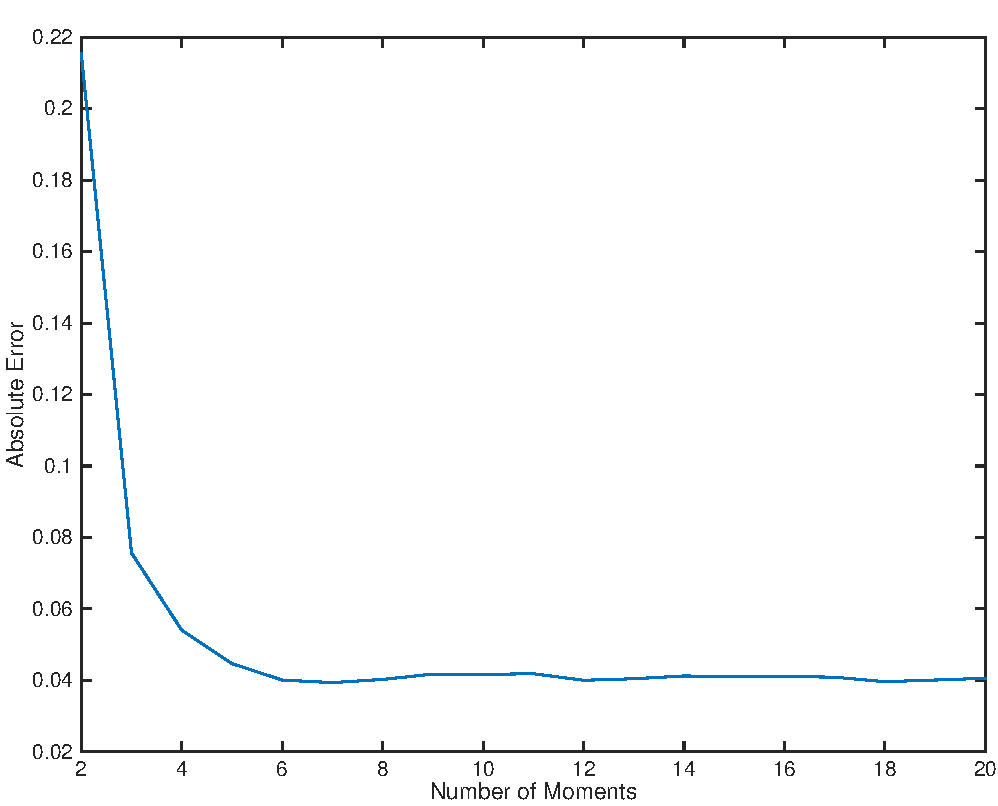
\includegraphics[width=0.5\textwidth]{thermo1smpmomer-cropped}
		\caption{Relative error against number of moments included for a single sample stochastic trace estimate for the Thermomech dataset. The corresponding graph for 50 samples is visually indistinguishable from this one.}
		\label{fig:thermomech1sampleerrorvsmoments}
	\end{figure}
	\begin{figure}[t]
		\centering 
		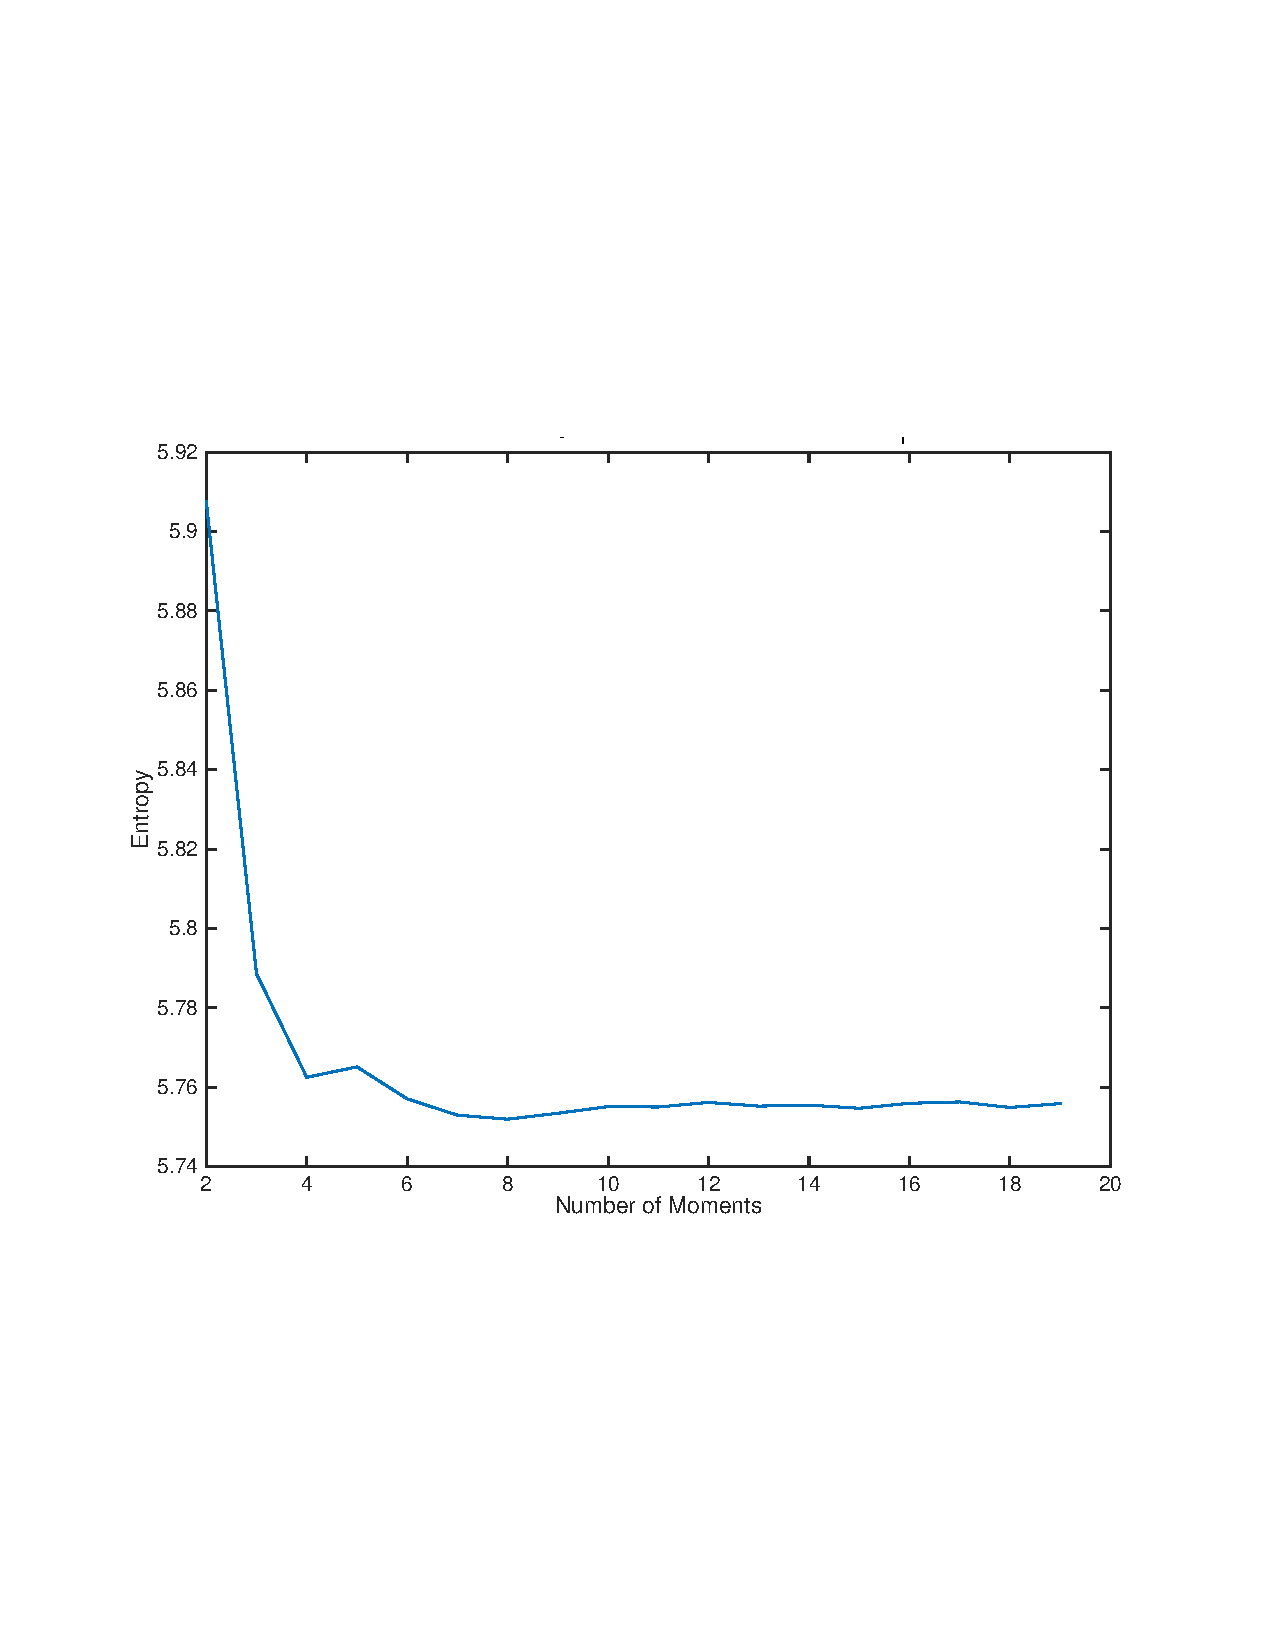
\includegraphics[width=0.5\textwidth]{cropped_thermomomentsentr}
		\caption{Entropy against number of Moments for the Thermomech dataset}
		\label{fig:thermoentropyvsmoments}
	\end{figure}
	
	
	
	% needed in second column of first page if using \IEEEpubid
	%\IEEEpubidadjcol
	
	% An example of a floating figure using the graphicx package.
	% Note that \label must occur AFTER (or within) \caption.
	% For figures, \caption should occur after the \includegraphics.
	% Note that IEEEtran v1.7 and later has special internal code that
	% is designed to preserve the operation of \label within \caption
	% even when the captionsoff option is in effect. However, because
	% of issues like this, it may be the safest practice to put all your
	% \label just after \caption rather than within \caption{}.
	%
	% Reminder: the "draftcls" or "draftclsnofoot", not "draft", class
	% option should be used if it is desired that the figures are to be
	% displayed while in draft mode.
	%
	%\begin{figure}[!t]
	%\centering
	%\includegraphics[width=2.5in]{myfigure}
	% where an .eps filename suffix will be assumed under latex, 
	% and a .pdf suffix will be assumed for pdflatex; or what has been declared
	% via \DeclareGraphicsExtensions.
	%\caption{Simulation Results}
	%\label{fig_sim}
	%\end{figure}
	
	% Note that IEEE typically puts floats only at the top, even when this
	% results in a large percentage of a column being occupied by floats.
	
	
	% An example of a double column floating figure using two subfigures.
	% (The subfig.sty package must be loaded for this to work.)
	% The subfigure \label commands are set within each subfloat command, the
	% \label for the overall figure must come after \caption.
	% \hfil must be used as a separator to get equal spacing.
	% The subfigure.sty package works much the same way, except \subfigure is
	% used instead of \subfloat.
	%
	%\begin{figure*}[!t]
	%\centerline{\subfloat[Case I]\includegraphics[width=2.5in]{subfigcase1}%
	%\label{fig_first_case}}
	%\hfil
	%\subfloat[Case II]{\includegraphics[width=2.5in]{subfigcase2}%
	%\label{fig_second_case}}}
	%\caption{Simulation results}
	%\label{fig_sim}
	%\end{figure*}
	%
	% Note that often IEEE papers with subfigures do not employ subfigure
	% captions (using the optional argument to \subfloat), but instead will
	% reference/describe all of them (a), (b), etc., within the main caption.
	
	
	% An example of a floating table. Note that, for IEEE style tables, the 
	% \caption command should come BEFORE the table. Table text will default to
	% \footnotesize as IEEE normally uses this smaller font for tables.
	% The \label must come after \caption as always.
	%
	%\begin{table}[!t]
	%% increase table row spacing, adjust to taste
	%\renewcommand{\arraystretch}{1.3}
	% if using array.sty, it might be a good idea to tweak the value of
	% \extrarowheight as needed to properly center the text within the cells
	%\caption{An Example of a Table}
	%\label{table_example}
	%\centering
	%% Some packages, such as MDW tools, offer better commands for making tables
	%% than the plain LaTeX2e tabular which is used here.
	%\begin{tabular}{|c||c|}
	%\hline
	%One & Two\\
	%\hline
	%Three & Four\\
	%\hline
	%\end{tabular}
	%\end{table}
	
	
	% Note that IEEE does not put floats in the very first column - or typically
	% anywhere on the first page for that matter. Also, in-text middle ("here")
	% positioning is not used. Most IEEE journals use top floats exclusively.
	% Note that, LaTeX2e, unlike IEEE journals, places footnotes above bottom
	% floats. This can be corrected via the \fnbelowfloat command of the
	% stfloats package.
	
	
	
	\section{Conclusion}
	In this paper we formally establish the link between sample expectation and mean value constraint, proving asymptotic equivalence. We also prove that the eigenvalue distribution of a Covariance matrix can be uniquely determined by its moments. The combination of these two provides a solid foundation for using stochastic trace estimation sample estimates as mean value constraints for a Maximum Entropy estimation of a Covariance matrix eigenvalue density.
	
	We further show how the inclusion of extra moment constraints, necessarily reduces the KL divergence $\mathbb{D}_{kl}(p||q)$ between the MaxEnt proposal $q(\lambda)$ and true eigenvalue spectrum $p(\lambda)$. We demonstrate empirically on SuiteSprase datasets how this reduction in $\mathbb{D}_{kl}(p||q)$ corresponds to increased estimation accuracy. 
	
	We investigate the effect of reducing the number of stochastic trace estimate samples empirically and experimentally demonstrate that the larger the matrix, the smaller the effect and the greater the computational benefit of reducing the number of samples. 
	
	We set up best practice guidelines, rooted in theory and experiment, for practitioners wishing to deal with large matrices. Our basic, non-optimized MaxEnt implementation is able to calculate determinants of $4$ million by $4$ million matrices on a laptop within a minute.
	
	% if have a single appendix:
	%\appendix[Proof of the Zonklar Equations]
	% or
	%\appendix  % for no appendix heading
	% do not use \section anymore after \appendix, only \section*
	% is possibly needed
	
	% use appendices with more than one appendix
	% then use \section to start each appendix
	% you must declare a \section before using any
	% \subsection or using \label (\appendices by itself
	% starts a section numbered zero.)
	%
	
	
	% use section* for acknowledgement
	\section*{Acknowledgments}
	The authors would like to thank the Oxford-Man Institute and the Royal Academy of Engineering for their support, Thomas Gunter and Michael Osborne for illuminating discussions, Pawan Kumar for his input on Convex Analysis and Tim Davies for the upkeep or the SuiteSparse dataset.
	
	% Can use something like this to put references on a page
	% by themselves when using endfloat and the captionsoff option.
	\ifCLASSOPTIONcaptionsoff
	\newpage
	\fi
	
	
	
	% trigger a \newpage just before the given reference
	% number - used to balance the columns on the last page
	% adjust value as needed - may need to be readjusted if
	% the document is modified later
	%\IEEEtriggeratref{8}
	% The "triggered" command can be changed if desired:
	%\IEEEtriggercmd{\enlargethispage{-5in}}
	
	% references section
	
	% can use a bibliography generated by BibTeX as a .bbl file
	% BibTeX documentation can be easily obtained at:
	% http://www.ctan.org/tex-archive/biblio/bibtex/contrib/doc/
	% The IEEEtran BibTeX style support page is at:
	% http://www.michaelshell.org/tex/ieeetran/bibtex/
	%\bibliographystyle{IEEEtran}
	% argument is your BibTeX string definitions and bibliography database(s)
	%\bibliography{IEEEabrv,../bib/paper}
	%
	% <OR> manually copy in the resultant .bbl file
	% set second argument of \begin to the number of references
	% (used to reserve space for the reference number labels box)
	
	
	% biography section
	% 
	% If you have an EPS/PDF photo (graphicx package needed) extra braces are
	% needed around the contents of the optional argument to biography to prevent
	% the LaTeX parser from getting confused when it sees the complicated
	% \includegraphics command within an optional argument. (You could create
	% your own custom macro containing the \includegraphics command to make things
	% simpler here.)
	%\begin{biography}[{\includegraphics[width=1in,height=1.25in,clip,keepaspectratio]{mshell}}]{Michael Shell}
	% or if you just want to reserve a space for a photo:
	
	
	% You can push biographies down or up by placing
	% a \vfill before or after them. The appropriate
	% use of \vfill depends on what kind of text is
	% on the last page and whether or not the columns
	% are being equalized.
	
	%\vfill
	
	% Can be used to pull up biographies so that the bottom of the last one
	% is flush with the other column.
	%\enlargethispage{-5in}
	
	
	
	% that's all folks
	\bibliographystyle{unsrt}%Used BibTeX style is unsrt
	\bibliography{sample}
\end{document}


